\chapter[Időlépéses program fejlesztése]{Időlépéses módszereket alkalmazó program fejlesztése}\label{chap: lin+nemlin progi}

{\ }

A következőkben az általam fejlesztett lineáris és nemlineáris időlépéses megoldó programokat mutatom be. A programokat MATLAB szoftverrel fejlesztettem, mert ez a programcsomag optimális választás a nagyméretű mátrixok gyors számítását igénylő feladatok esetében. Az egyes programokat eleve műveleti blokkokra osztottam, hogy a később bemutatásra kerülő hibrid módszert alkalmazó program elemeit könnyebb legyen beilleszteni. Az egyes műveleti blokkok a  feladatuk tekintetében megfeleltethetők egymásnak a  lineáris időlépéses megoldó, a nemlineáris időlépéses megoldó és a hibrid szimulációs  programban is. A lineáris és nemlineáris  időlépéses megoldó programok verifikálása a következő  fejezetben   olvasható.  Az egyes programok forráskódjait a Függelék tartalmazza.

\section{Lineáris feladatok megoldására fejlesztett program bemutatása}\label{sec: lin progi}

{\ }

A lineáris feladatok megoldására alkalmazható időlépéses megoldó módszereket használó program feladata elsősorban a \ref{sec:idolepmsz} pontban ismertetett időlépéses módszerek alkalmazása adott feladatokra, illetve az ezen algoritmusok összehasonlítása a módszer stabilitása, a megoldás pontossága valamint a számítások lefutásának sebessége szerint. A programban saját megoldó algoritmusokat használok.

\subsection{A program szerkezete}\label{subsec: lin prog szerk}

{\ }

A program folyamatábrája a \ref{fig:linprog} ábrán látható. Az indítást megelőzően szükséges  a szerkezeti rendszert leíró mátrixok és a kezdeti feltételek kézi megadása, valamint az egyes algoritmusokhoz tartozó integrálási paraméterek beállítása. Az indítást követően a program először létrehozza a  vizsgált rendszert leíró mátrixokat. Ezután egy felugró menüben ki kell választani az alkalmazni kívánt integráló algoritmust. A program ezt követően inicializálja a kiválasztott módszerhez tartozó integrálási paramétereket (ha van ilyen), majd létrehozza, illetve kiszámítja a módszerhez szükséges, a vizsgálat közben állandó (így csak egyszer előállítandó, esetleg invertálandó) segédmátrixokat, továbbá lefoglalja a helyet az időlépésenként  számítandó mátrixoknak. Ekkor egy for ciklusban az előre megadott vizsgálati időintervallumban, előre beállított lépésközökkel időlépésenként kiszámítja az elmozdulásvektort a kiválasztott módszer algoritmusával, majd el is tárolja azt. Végül a program kirajzolja az eredményül kapott diszkrét elmozdulásvektorokat a vizsgálat teljes időintervallumára.  
 
\begin{figure}[h!]
\centering
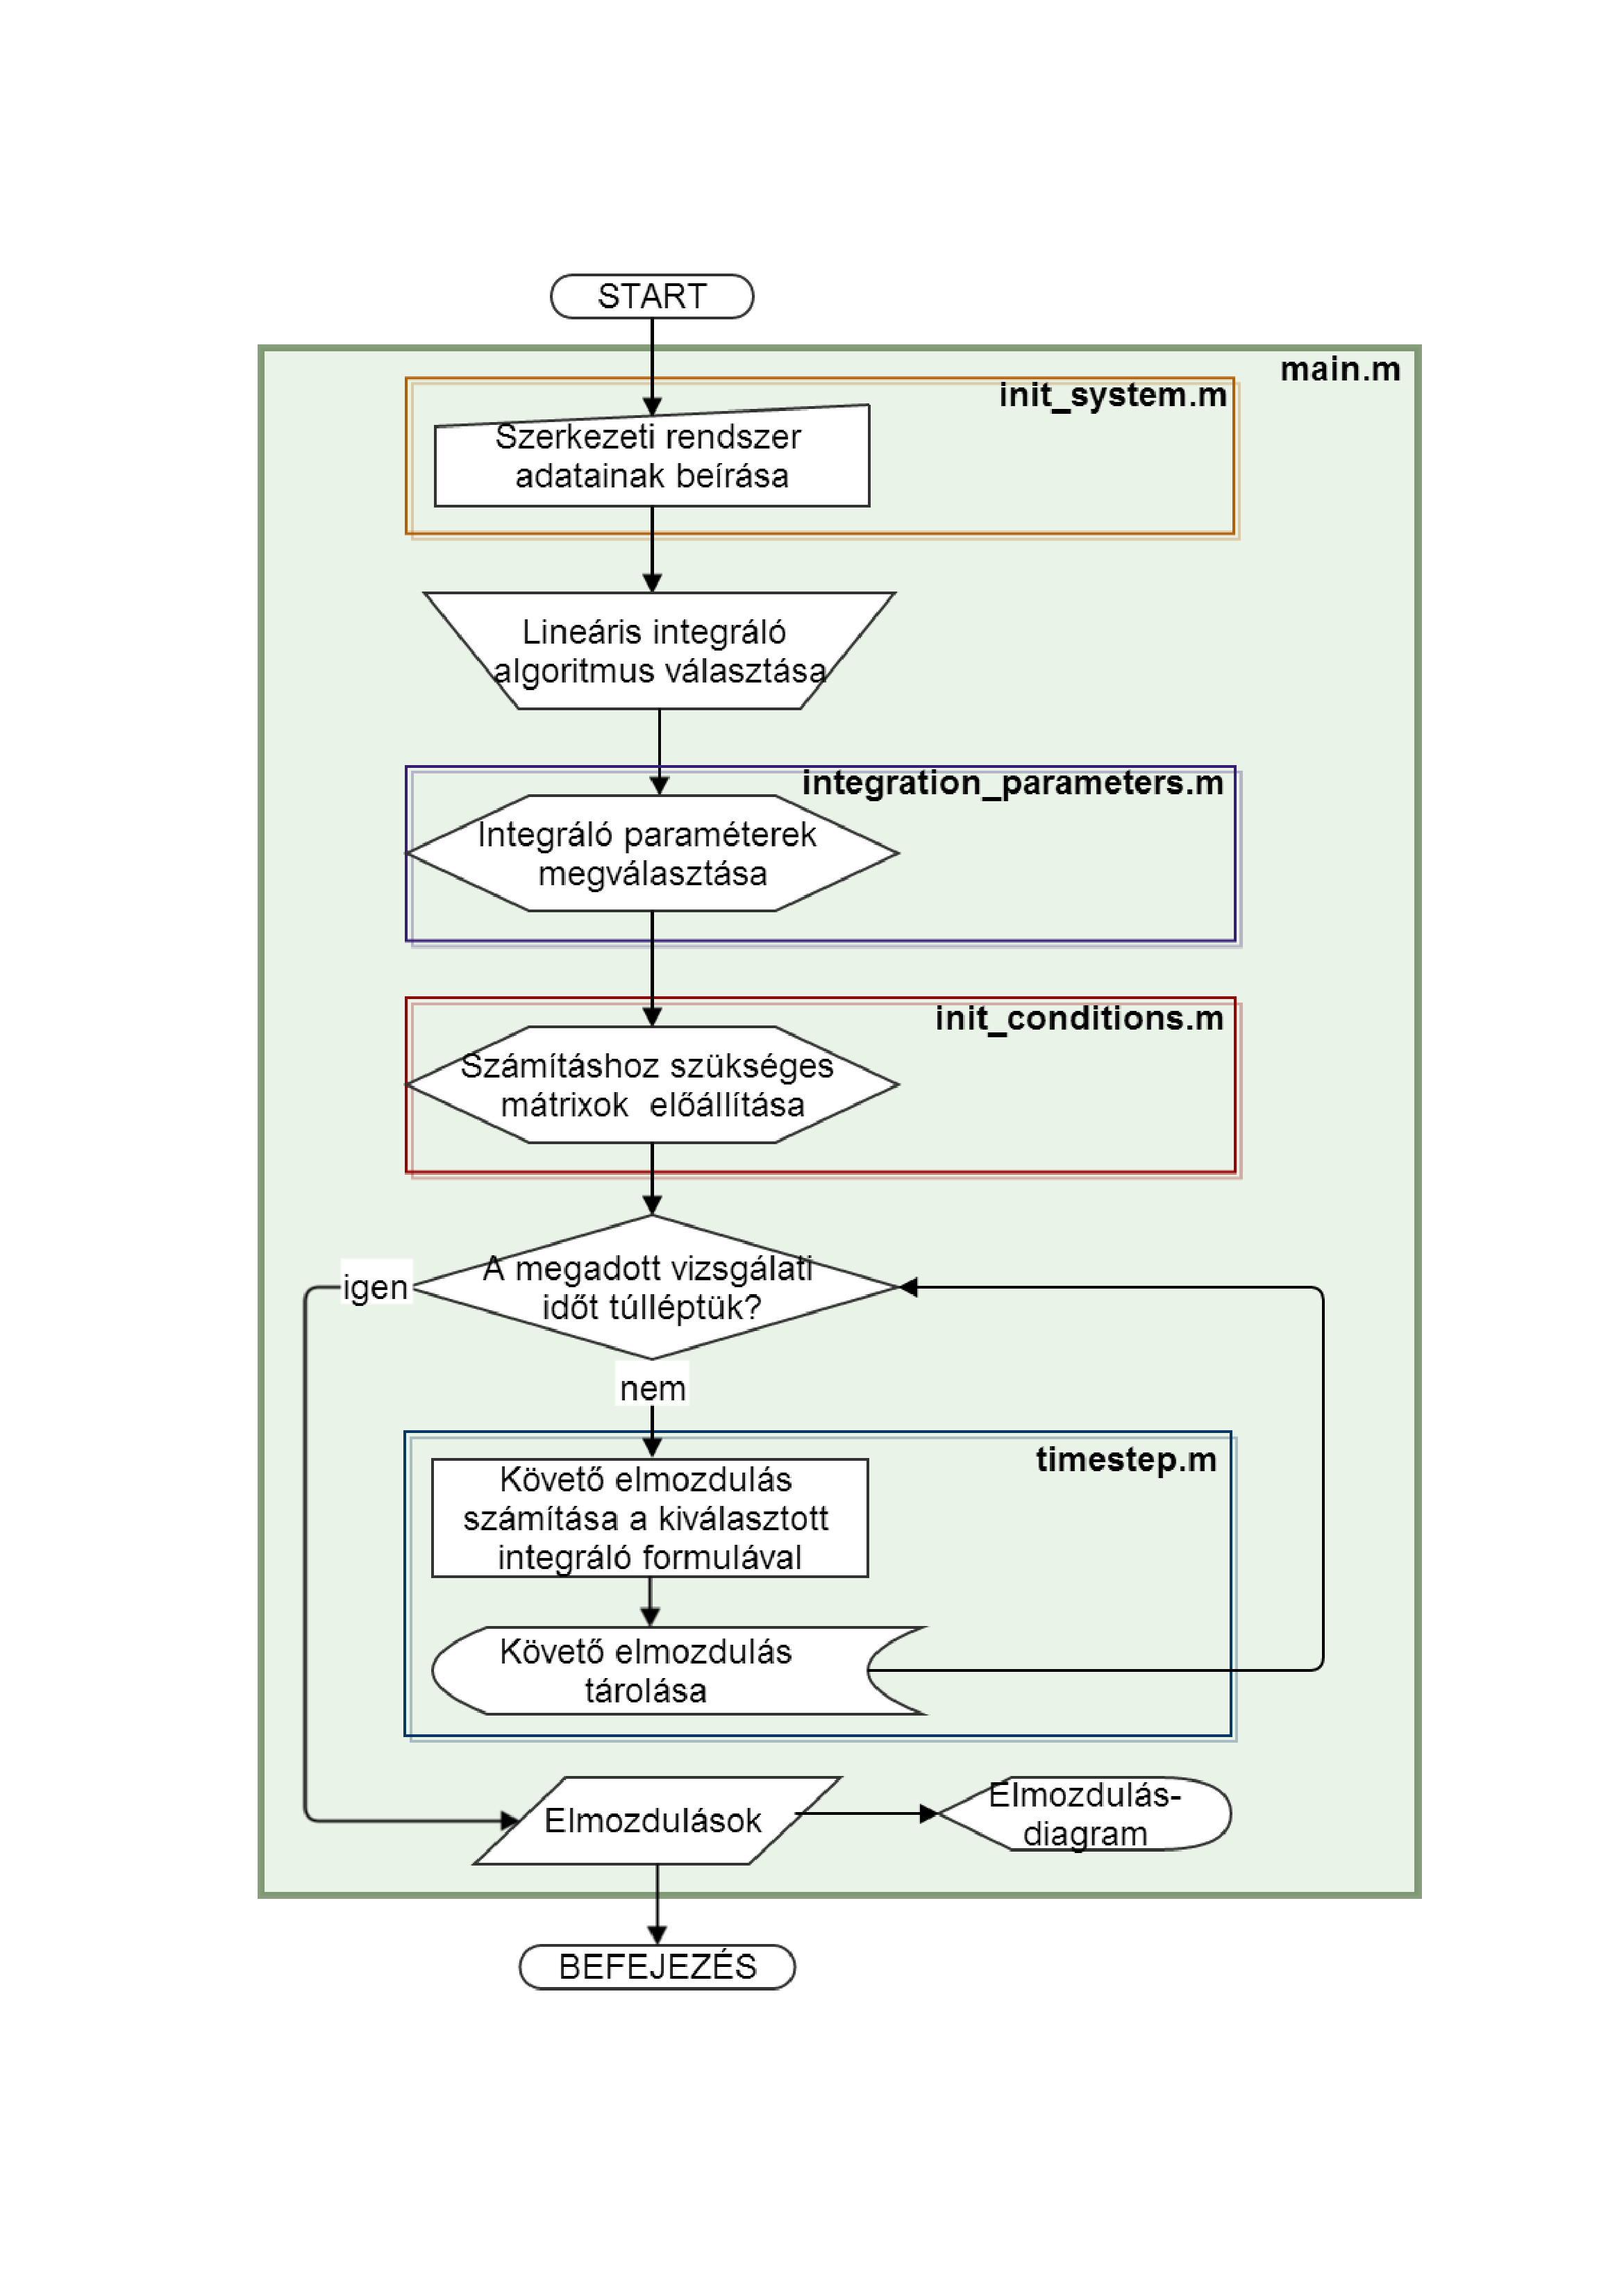
\includegraphics[trim = 0mm 50mm 0mm 50mm, clip, width=\textwidth]{linearis_folyamatabra.pdf}
\caption{A lineáris időlépéses megoldó program folyamatábrája.}
\label{fig:linprog}
\end{figure}

A program műveleti blokkokból áll. Teljes kódja a Függelék \ref{chap: függ linprog}. pontjában található. A szkript típusú \verb|main.m| fájl tartalmazza a műveleti parancssort és a beillesztett inicializáló és számító blokkokat egyaránt.  Először egy biztonsági törlés elvégzését követően meghívja az \verb|init_system.m| fájlt a szerkezet alapadatainak beolvasásához. A main tartalmazza a felugró menüt, amiben a numerikus algoritmust választhatjuk ki. A módszer kiválasztása után futtatja az \verb|integration_parameters.m| valamint \verb|init_conditions.m| szkripteket, melyek az algoritmus futásához szükséges előkészületeket végzik. Ezt követően egy for ciklusban hívja a \verb|timestep.m| fájlt az elmozdulások számításához, majd kirajzolja az eredményt egy elmozdulás-idő grafikonon. 

A szerkezetet leíró mátrixokat és a kezdeti feltételeket az \verb|init_system.m| fájlban kell megadni. Ezek a vizsgálat időtartama, a diszkrét időpillanatok lépésköze, a szerkezetet leíró tömeg-, merevségi és csillapítási mátrixok, a tehervektor, illetve az $\mathbf{u}_0$ és  $\mathbf{\dot{u}}_0$  kezdeti feltételek. Ha az adott feladatban szükséges, számítjuk a szerkezet sajátkörfrekvenciáit és sajátrezgésalakjait.

Az egyes módszerekhez tartozó integrálási paraméterek értékeit (ha van ilyen) az \verb|integration_parameters.m| fájlban lehet beállítani. Ezek a  Newmark eljárásnál  $\gamma$ és $\beta$, a Wilson-$\theta$ eljárásnál $\theta$, a HHT-$\alpha$ módszernél $\gamma$, $\beta$ és $\alpha$, valamint a CR algoritmus esetében $\boldsymbol\alpha_1$ és $\boldsymbol\alpha_2$ paraméterek. Az egyes módszerek stabilitásához szükséges értékeket kommentként feltüntettem.
 
Az \verb|init_conditions.m| szkript tartalmazza a helyfoglaló mátrixokat, mint az elmozdulás-, sebesség- és gyorsulásvektorok mátrixait, továbbá elvégzi az egyes módszerekhez szükséges előre elvégezhető mátrixszámításokat, például a hatékony tömeg- vagy merevségi mátrix invertálását. 

 A \verb|timestep.m| fájlban pedig  az elmozdulásvektorok számítására  és tárolására vonatkozó, minden időlépésben végrehajtandó parancsok találhatók a \ref{sec:idolepmsz} pontban ismertetett algoritmusok alapján.
 
A program használatát két példán keresztül mutatom be. Mindkét esetben csak az \verb|init_system.m| fájlt kell a feladathoz igazítani és a "main" paranccsal meghívni a főprogramot, majd kiválasztani az integrálási algoritmust. 


\subsection{A program használata gerjesztett rezgés vizsgálatára}\label{subsec:lingerj}

{\ }

Ezen a példán keresztül három dolgot prezentálok. Bemutatom, hogyan adhatunk meg a programban  gerjesztést, hogyan állíthatunk be egy lecsengő szakaszon csillapított szabadrezgést, valamint hogy hogyan vizsgálhatjuk a gerjesztés és a csillapítás hatását. 

\begin{figure}[h!]
\centering
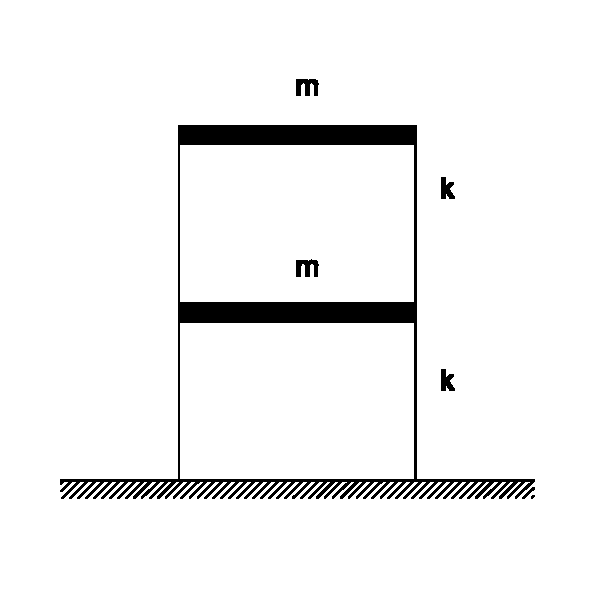
\includegraphics[width=0.4\textwidth]{ketzsintes.pdf}
\caption{A gerjesztéses példában vizsgált kétszintes keret.}
\label{fig:ketszabfok}
\end{figure}

A feladatban egy kétszabadságfokú rendszert gerjesztünk 6 másodpercig harmonikus gerjesztőerővel zérus kezdeti feltételek mellett, ekkor megszüntetjük a terhelést, és megvárjuk, amíg a szerkezet szabadrezgéssel lecsillapodik. Így az első szakaszban a  gerjesztés hatását, a második szakaszban pedig a csillapítás hatását tudjuk szemügyre venni. 

A modell egy kétszintes szerkezet, az egyes szintek tömege 45 tonna. Az egyes szintek merevsége 18000 kN/m. A  szerkezeten arányos csillapítást alkalmazunk, $\alpha$ és $\beta$ értékét úgy vesszük fel, hogy mindkét módban $\xi$ tényező értéke $5\%$ legyen. A lépésközt úgy választjuk meg, hogy megfeleljen az erre vonatkozó ökölszabálynak, és a 6 másodperc osztója legyen. Ez alapján a $dt = 0.02 s$ értéket vesszük fel. A teherfüggvény  az első 6 másodpercben mindkét szinten $10\sin(20t)$, utána zérus. A rendszert leíró bemeneti értékek képletekkel megadva a következők:
  \begin{align*}
  & t_{max}  = 12 sec  & & \Delta{t} = 0,02 sec   & \\
  & \mathbf{M}  = \left[\begin{array}{rr}  45 & 0 \\ 0 & 45 \end{array} \right]t   &  & \mathbf{K} = \left[\begin{array}{rr} 36 000 & -18 000 \\ -18 000 & 18 000 \end{array} \right]\frac{kN}{m}  &  \\
  & \mathbf{C}  = \alpha\mathbf{M}+\beta\mathbf{K}  &  & \xi = 0,05  & \\
  & \mathbf{q}_1  = \left[\begin{array}{c} 10 \\ 10 \end{array} \right]\sin{20t}  & & \mathbf{q}_2 = \left[\begin{array}{c} 0 \\ 0 \end{array} \right]  & \\
  & \mathbf{u}(0)  = \left[\begin{array}{c} 0 \\ 0 \end{array} \right]  & & \mathbf{\dot{u}}(0) = \left[\begin{array}{c} 0 \\ 0 \end{array} \right] & 
  \end{align*}
  %& \left[ \begin{array}{c} \alpha \\ \beta \end{array} \right] =  \left[ \begin{array}{c} \frac{2\xi\omega_{01}\omega_{02}}{\omega_{01}+\omega_{02}} \\ \frac{2\xi}{\omega_{01}+\omega_{02}} \end{array} \right], &

A programban ez alapján a  feladathoz tartozó \verb|init_system.m| fájl a következő: 
\lstinputlisting{"MATLAB/linear_system_312/init_system.m"}

A program az elmozdulásokat rajzolja ki az idő függvényében. A feladat Newmark eljárással való megoldása látható a \ref{fig:lingerjeredm_newmark} ábrán. A grafikon alapján elmondható, hogy a rendszer a gerjesztés alatt közel beáll egy állandósult rezgésre. Majd mikor megszüntetjük a gerjesztőerőt, kap egy nagyobb sebességet, aminek következtében megjelenik egy nagyobb kitérés. Ezt egy lecsengő szakasz követi, a csillapított szabadrezgésnek megfelelően. 
\begin{figure}[h!bt]
\centering
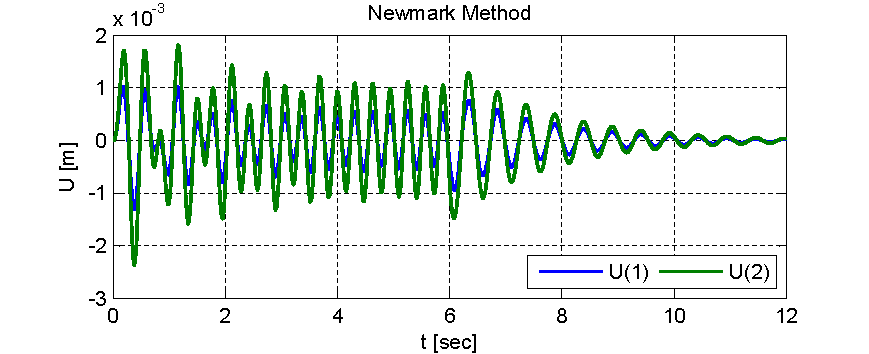
\includegraphics[width=\textwidth]{312_Newmark.pdf}
\caption{A \ref{subsec:lingerj} gerjesztett rezgéses példa elmozdulásai Newmark módszerrel.}
\label{fig:lingerjeredm_newmark}
\end{figure}

A számítás eredményei a többi módszerrel  a Függelék \ref{sec:függ_lingerj} pontjában találhatók. Ezeket a \ref{subsec: lin eredmény gerj} pontban hasonlítom össze.


\subsection{A program használata csillapítatlan szabadrezgés vizsgálatára}\label{subsec:szabrezg}

{\ }


E feladat célja az egyes módszerek jellemzése stabilitás és pontosság szempontjából. A csillapítás megszüntetésével az egyes módszerek stabilitása közelítő módon, numerikusan vizsgálható. Ahhoz, hogy az egyes rezgésmódok ne zavarják a szerkezet viselkedését, a  kezdeti feltételt valamelyik sajátalakként célszerű felvennünk.

Csillapítatlan szabadrezgés vizsgálatához a \ref{subsec:lingerj} pontban bemutatott kétszabadságfokú rendszert választottam. A feladatban a csillapítás és a tehervektor értéke egyaránt zérus, kezdeti feltételnek pedig az egyik sajátvektorral arányos kitérést adtam meg. A rendszert leíró bemeneti értékek a következőképp módosulnak a  gerjesztett rezgéshez képest:
  \begin{align*}
    & \mathbf{C}  = 0  & & \mathbf{q} = \left[\begin{array}{c} 0 \\ 0 \end{array} \right]  & \\
  & \mathbf{u}(0)  = \mathbf{v}_1  & & \mathbf{\dot{u}}(0) = \left[\begin{array}{c} 0 \\ 0 \end{array} \right]  & 
  \end{align*}
  
A bemeneti adatokat tartalmazó \verb|init_system.m| a következőkben módosul:
\lstinputlisting{"MATLAB/linear_system_313/init_system.m"}
 

\begin{figure}[h]
\centering
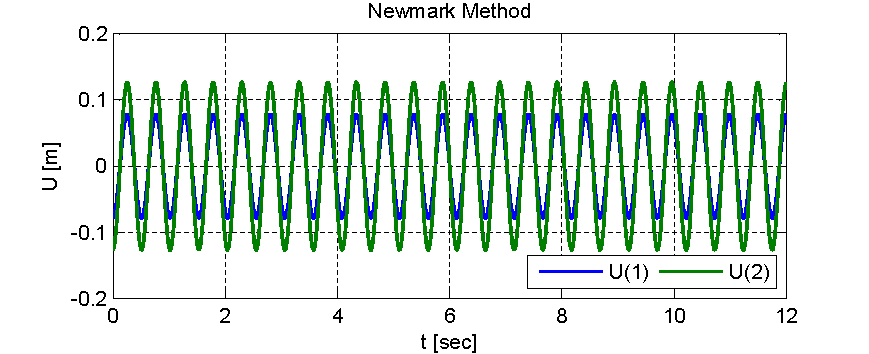
\includegraphics[width=\textwidth]{313_Newmark.pdf}
\caption{A \ref{subsec:szabrezg} szabadrezgéses példa elmozdulásai Newmark módszerrel.}
\label{fig:szabrezg_er_newmark}
\end{figure}

A \ref{fig:szabrezg_er_newmark} ábrán a feladat megoldásaként az elmozdulás-idő diagram látható, Newmark eljárással számítva. 
A pontosság szemléltetésére  a diagram nem feltétlenül alkalmas, mert az amplitúdó csökkenése a legtöbb esetben a görbén nem látszik egyértelműen, azonban a többi módszer eredményeivel összehasonlítva megfigyelhető rajta a periódusidő meghosszabbodása.  A programmal az elmozdulás-idő grafikon mellett kirajzoltattuk a mechanikai energia-idő diagramot, valamint a szerkezet két szintjének egymáshoz viszonyított  elmozdulását fázistérben. Erre egy-egy  példát  láthatunk Newmark módszerrel számítva a \ref{subsec: lin eredmény szabrezg} pontban.

 

\section{Nemlineáris feladatok megoldására fejlesztett program bemutatása}\label{sec: nemlin progi}

{\ }

A nemlineáris feladatok megoldására használható  programot szintén MATLAB programnyelven fejlesztettem. A program feladata  a \ref{sec:nl idolepmsz} pontban bemutatott időlépéses integráló formulák alkalmazása nemlineáris szerkezetekre, illetve ezen algoritmusok pontosságának. Ebben a programban is saját megoldó algoritmusokat használok.


\subsection{A program szerkezete}\label{subsec: nemlin prog szerk}
 
{\ }

A program folyamatábráját mutatja a \ref{fig:nemlinprog} ábra. A szerkezeti rendszer adatait és a kezdeti feltételeket a nemlineáris programban is az indítást megelőzően, kézzel kell  megadni. A Newmark algoritmusok használata esetén ekkor kell beállítani az integráló paraméterek értékét is. A program az indítását követően először létrehozza a szerkezeti rendszert leíró mátrixokat. Ezt követően egy felugró menüben kiválaszthatjuk az integráló algoritmust. Ekkor a Newmark algoritmusok esetében a integrálási paraméterek inicializálása következik, majd a választott módszer algoritmusához időlépésenként számítandó mátrixok helyfoglalása  és  a vizsgálat közben állandó kifejezések segédmátrixainak előállítása és tárolása történik. Ezután az időlépésekhez tartozó for ciklus következik. Minden lépésnél frissítjük a visszatérítő erőt és a Newmark formulák esetében az érintőmerevség értékét is, kiszámítjuk a következő időpillanatbeli elmozdulást, és eltároljuk az eredményt. Az utolsó lépés az eredményül kapott  elmozdulásvektor-diagramok kirajzolása a vizsgálat teljes idejére. 
 
\begin{figure}[h!]
\centering
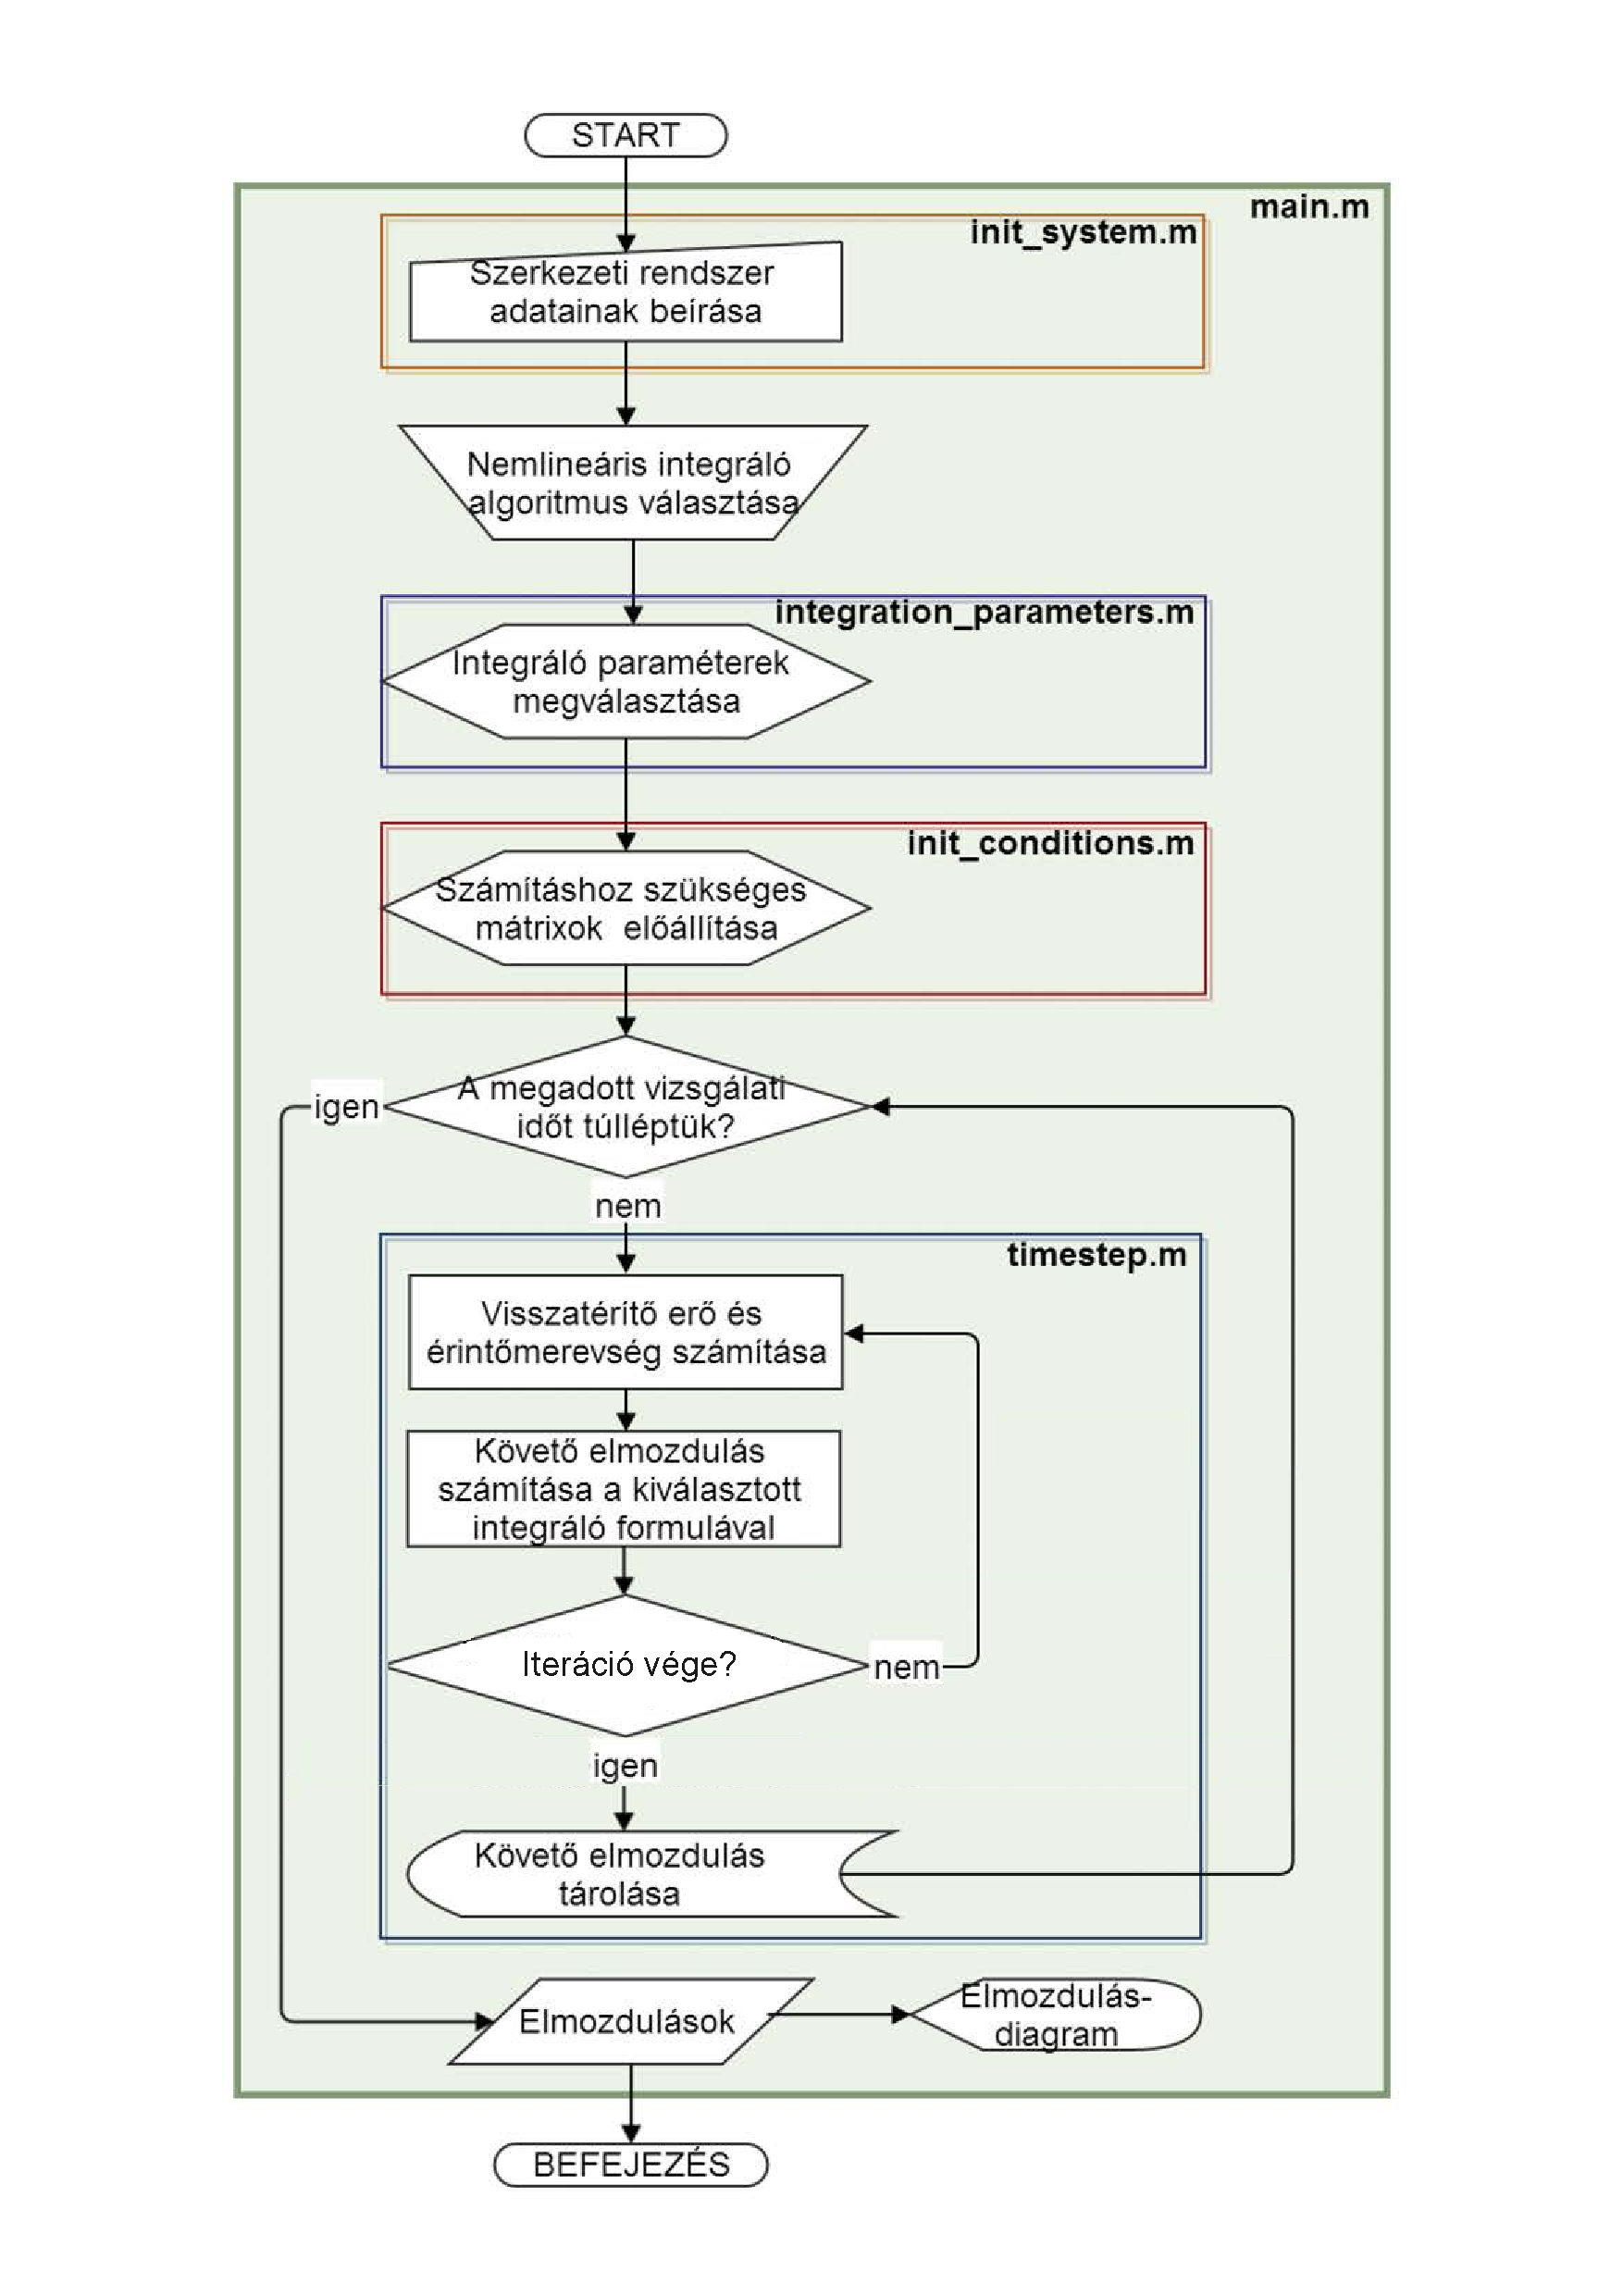
\includegraphics[ width=\textwidth]{nemlinearis_folyamatabra.pdf}
\caption{A nemlineáris időlépéses megoldó program folyamatábrája.}
\label{fig:nemlinprog}
\end{figure}

A nemlineáris megoldó program szintén műveleti blokkokból áll, ezek közül néhány blokk feladata összeegyeztethető a lineáris programnál a \ref{subsec: lin prog szerk} pontban bemutatott szkriptekével. A teljes programkód a Függelék \ref{chap: függ nemlinprog}. pontjában található. A  műveleti parancssort és az inicializáló és számító blokkokat a \verb|main.m| fájl tartalmazza. Indításkor egy biztonsági törlés elvégzése után meghívja az \verb|init_system.m| szkriptet a szerkezet adatainak beolvasására. Ezt követi a felugró menü, amiben a használandó nemlineáris integráló algoritmust választhatjuk ki. A main az egyik Newmark eljárás választása esetén futtatja  az integráló paraméterek és az iterációk adatainak inicializálására az \verb|integration_parameters.m| szkriptet az integráló paraméterek és az iterációk adatainak inicializálására, majd hívja az \verb|init_conditions.m| fájlt a kiválasztott algoritmushoz tartozó helyfoglaló és  előre definiálható segédmátrixok előállítására. Ezt az időlépésekhez tartozó for ciklus követi. A ciklusban a \verb|timestep.m| szkript számolja az időlépésenkénti érintőmerevséget, és (Newmark eljárásoknál kvázi-Newton-Raphson iterációt alkalmazva) a visszatérítő erőt is, valamint ezek segítségével a következő időpontbeli elmozdulást. Végül a main kirajzolja az eredményeket egy elmozdulás-idő diagramon.

 A vizsgált szerkezet adatai az \verb|init_system.m| fájlban találhatók. Ezek a vizsgálat időtartama, a diszkrét időpillanatok lépésköze, a szerkezetet leíró tömeg-, merevségi és csillapítási mátrixok, a tehervektor,  az $\mathbf{u}_0$ és  $\mathbf{\dot{u}}_0$  kezdeti feltételek, valamint a visszatérítő erő és az érintőmerevség számításokhoz szükséges kezdeti értékek és globális változók. Ha az adott feladatban szükséges, szintén itt számítjuk a szerkezet sajátkörfrekvenciáit és sajátrezgésalakjait.
 
 A Newmark algoritmusoknál használt integrálási paramétereket, valamint  a kvázi-Newton-Raphson iteráció adatait  az \verb|integration_parameters.m| fájlban lehet beállítani.  Ezek a $\gamma$ és a $\beta$ paraméterek,  az iterációk száma és az iteráció leállásához szükséges  kritérium feltétel. 
 
 Az \verb|init_conditions.m| szkript hozza létre a kiválasztott algoritmushoz tartozó helyfoglaló mátrixokat mint az elmozdulás-, a sebesség- és a gyorsulásvektorok mátrixát, és az  előre definiálható segédmátrixokat. Centrális differenciák módszere esetén elvégzi a hatékony tömegmátrix invertálását.
 
 A \verb|timestep.m| szkriptben az időlépésekhez tartozó számítások parancssora található. A fájl végzi a visszatérítő erő és  az érintőmerevség frissítését. A Newmark formulák esetében kvázi-Newton-Raphson iterációval számítja a következő  időpillanatbeli elmozdulásokat, és az iterációt követően  tárolja  az eredményeket.

A nemlineáris program futásához szükség van a visszatérítő erő és az érintőmerevség időlépésenkénti számítására. A visszatérítő erő számítása a  \verb|resisting_force.m|, az érintőmerevségé pedig a  \verb|tangent_stiffness.m| függvényfájlokkal történik, ezek tartalmazzák  a nemlineáris  viselkedést leíró függvényeket. A nemlineáris anyagmodell módosítása  ebben a két fájlban egyszerűen megoldható. A számításhoz szükséges globális változókat az \verb|init_system.m| szkriptben adjuk meg.

A program használatát bemutatom statikus probléma vizsgálatára, több csillapítási tényező értéket figyelembe véve, majd  alkalmazom a programot dinamikus probléma vizsgálatára különböző terhelések mellett. 
 
\subsection{A program használata statikus  probléma vizsgálatára} \label{subsec:nemlinstat}

Nem írtam külön programot a statikus nemlineáris feladatok vizsgálatára, de a dinamikus vizsgálatra fejlesztett program is használható erre a célra. Ehhez a teherfüggvényt konstans értékűre kell felvenni, és megfelelően nagy csillapítást kell alkalmazni. A feladat a teherszintek nemlineáris hatásának összehasonlítására alkalmazható.

A feladatban a \ref{subsec:lingerj} pontban bemutatott kétszabadságfokú szerkezetet vizsgáljuk, azonban a csillapítás és a teherfüggvény eltérő, és a szintenkénti merevség  nemlineáris. A megfelelően nagy csillapítás bemutatására különböző $\xi$ paramétereket alkalmaztam.
\begin{align*}
\mathbf{q} & = \mathbf{q}_0 \cos{0t} \\
\mathbf{C} & = \alpha\mathbf{M}+\beta\mathbf{K}  &   \xi & = 0,1 ; 0,5 ; 1,1 
\end{align*}

Az anyagi nemlinearitást  egy arkusz tangens függvénnyel vettem figyelembe.  Azért ezt választottam, mert látványosan nemlineáris, de rugalmas modell, és a lineáris modellhez képest nagyon nagy eltérést mutat nagy alakváltozások esetében. Azonban megjegyezném, hogy ez az anyagmodell  fiktív. A visszatérítő erő és az érintőmerevség: 
\begin{align*}
f_s(\Delta{l}) & = a \arctan{b\Delta{l}}, \\
k_T & = \frac{\delta\mathbf{f}_s}{\delta\Delta{l}} = \frac{ab}{1+b^2\Delta{l}^2},
\end{align*}
ahol $a$ és $b$ paramétert úgy választottuk, hogy a kezdeti időpillanatban az érintőmerevség mindkét szinten $k_{T,0} = 18000 \frac{kN}{m}$, azaz a lineáris rendszer merevségével megegyező legyen. 

Az \verb|init_system.m| fájlban a következő eltérések vannak:

\lstinputlisting{"MATLAB/nonlinear_system_322/init_system.m"}

A \verb|resisting_force.m| és a \verb|tangent_stiffness.m| függvények a következők:

\lstinputlisting{"MATLAB/nonlinear_system_322/resisting_force.m"}
\lstinputlisting{"MATLAB/nonlinear_system_322/tangent_stiffness.m"}



\begin{figure}[h!]
\centering
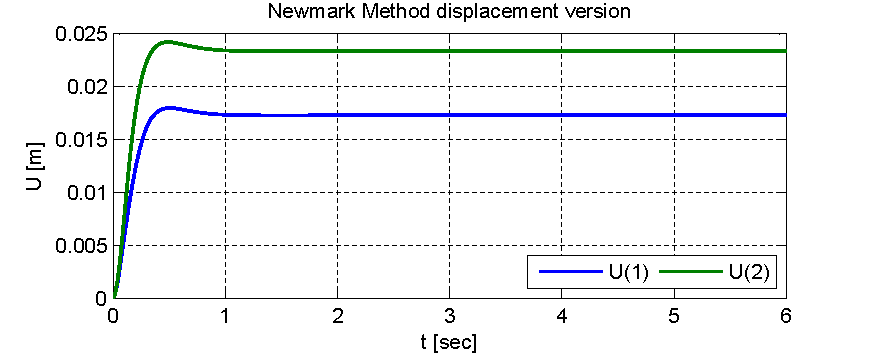
\includegraphics[width=\textwidth]{322_newmark_disp_kszi_0_5.pdf}
\caption{A \ref{subsec:nemlinstat} statikus probléma elmozdulásai a Newmark módszer elmozdulásos változatával, $\xi = 0,5$  esetén.}
\label{fig:322_newmark_disp_0_5}
\end{figure}

A feladat megoldása a Newmark módszer elmozdulásos változatával a \ref{fig:322_newmark_disp_0_5} elmozdulás - idő grafikonon látható. A csillapítás értéke $\xi = 0,5$-del van figyelembe véve. Ez kellően nagy csillapításnak számít, ekkora  mellett már gyorsan lecsillapodik a rezgés. Az eredményeket a \ref{subsec: nemlin eredmény stat} pontban elemzem. A többi csillapításértékkel számított elmozdulások grafikonjai is ebben a  pontban láthatók. 


\subsection{A program használata dinamikus probléma vizsgálatára} \label{subsec:nemlindin}

Ebben a feladatban a dinamikus nemlineáris viselkedést szeretném bemutatni. A  példában szintén a \ref{subsec:lingerj} pontban bemutatott kétszabadságfokú szerkezetet vizsgáljuk. Az anyagmodell megegyezik a \ref{subsec:nemlinstat} statikus problémánál ismertetettel. A szerkezetet különböző amplitúdójú szinuszos terhelésre vizsgáljuk, és összehasonlítjuk az elmozdulásait a terhek függvényében. Az amplitúdók rendre 10, 20, 40 és 80kN. A csillapítás $\xi = 0,05$ paraméterrel van figyelembe véve. 
 
\begin{align*}
\mathbf{q} & = \left[\begin{array}{cc}\mathbf{q}_0\\ \mathbf{q}_0 \end{array}\right] \sin{20t} & \mathbf{q}_0 & = 10; 20; 40; 80 kN\\
\mathbf{C} & = \alpha\mathbf{M}+\beta\mathbf{K}  &   \xi & = 0,05 
\end{align*}

% \lstinputlisting{"MATLAB/nonlinear_system_323/init_system.m"}
% \lstinputlisting{"MATLAB/nonlinear_system_323/resisting_force.m"}
% \lstinputlisting{"MATLAB/nonlinear_system_323/tangent_stiffness.m"}

\begin{figure}[h!]
\centering
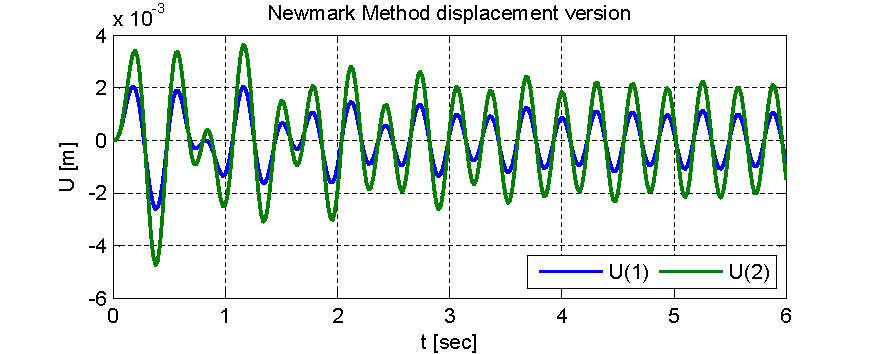
\includegraphics[width=\textwidth]{323_Newmark_disp.pdf}
\caption{A \ref{subsec:nemlindin} dinamikus probléma elmozdulásai a Newmark módszer elmozdulásos változatával, $\mathbf{q}_0 = 20$ esetén.}
\label{fig:323_newmark_disp}
\end{figure}

A \ref{fig:323_newmark_disp} ábrán az elmozdulás - idő diagram látható a Newmark módszer elmozdulásos változatával számolva, $\mathbf{q}_0 = 20$ amplitúdójú teherrel. A program kirajzolja a különböző terhelésekkel számolt elmozdulásokat egy ábrára is, így megfigyelhető, milyen összefüggés van a terhelés és az elmozdulás amplitúdója között. Az eredményeket a \ref{subsec: nemlin eredmény din} pontban mutatom be. 


\section{Az időlépéses módszerek összehasonlítása a programok eredményei alapján}\label{sec: msz összehasonlítás}

\subsection{A lineáris időlépéses megoldó program eredményei gerjesztett rezgés esetén}\label{subsec: lin eredmény gerj}

{\ }

A \ref{subsec:lingerj} gerjesztéses feladat alapján összehasonlíthatók az egyes időlépéses módszerek. Az eredmények a Függelék \ref{sec:függ_lingerj} pontban találhatók. 

Az Euler - módszer ábráján az látszik, hogy a megoldás instabillá vált, az elmozdulások a végtelenbe tartanak. A többi grafikon nagyjából hasonló eredményt mutat, nincs másik kirívó eset.

A dinamikus hatás szemléltetésére kirajzoltattam az elmozdulást az $\mathbf{u}_{st}(t) = \mathbf{K}_0^{-1}\mathbf{q}(t)$ statikus elmozdulással együtt az idő függvényében (\ref{fig:lingerjeredm_newmark_Ku} ábra). Az ábrán jól látható, hogy a szerkezet a terheléssel ellentétes fázisban rezeg, hiszen $\omega > \omega_{01}$, és főleg az első alak van gerjesztve a teherfüggvénnyel.

\begin{figure}[H]
\centering
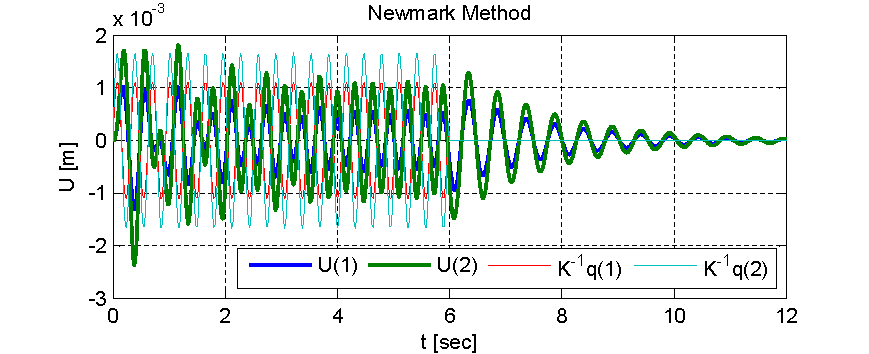
\includegraphics[width=\textwidth]{312_Newmark_Ku.pdf}
\caption{A \ref{subsec:lingerj} gerjesztett rezgéses példa elmozdulásai Newmark módszerrel és a statikus elmozdulás.}
\label{fig:lingerjeredm_newmark_Ku}
\end{figure}



\subsection{A lineáris időlépéses megoldó program eredményei csillapítatlan szabadrezgés esetén}\label{subsec: lin eredmény szabrezg}

{\ }

 A \ref{subsec:szabrezg} szabadrezgéses feladat alapján vizsgálható az egyes időlépéses módszerek stabilitása és pontossága. A \ref {fig:szabrezg_erek_newmark-a} ábrán a rendszer mechanikai energiája, a \ref{fig:szabrezg_erek_newmark-b} grafikonon pedig a fázistérben ábrázolt elmozdulásai láthatók. Az program által kirajzolt  eredmények  a többi módszerrel a Függelék \ref{sec:függ_szabrezg}.  pontjában találhatók. 
 
 A feladatban vizsgálhatjuk az elmozdulást az idő függvényében, és  következtethetünk a periódusidők meghosszabbodására. Azonban a diagramon az amplitúdó változások kicsik,  és a maximumok pontos értéke nehezen érzékelhető, ezért   nehéz ezeket  leolvasni.  A probléma megoldására kirajzoltattam  a mechanikai energiát diszkrét $t_i$ időpontokban, valamint a szabadságfokok elmozdulásának arányát. A mechanikai energiának ekkor nem szabad növekednie stabil rendszereknél, az elmozdulások arányának pedig a fázistér vetületében egyenesnek kell lennie.  
 
A szerkezet mechanikai energiáját a következő képlettel számíthatjuk:
\[ E_m = \frac{1}{2}\mathbf{u}_i^T\mathbf{K}\mathbf{u}_i+\frac{1}{2}\mathbf{u}_i^T\mathbf{M}\mathbf{u}_i\]
Ennek számítását a programkódban a  \verb|main.m| fájlban a következőképp deklaráltam:

  \mcode{ME(:,i) = 1/2*(U(:,i).'*K*U(:,i))+1/2*(dU(:,i).'*M*dU(:,i));}.
  

\begin{figure}[h!b]%
\centering
\subfigure[][]{%
\label{fig:szabrezg_erek_newmark-a}%
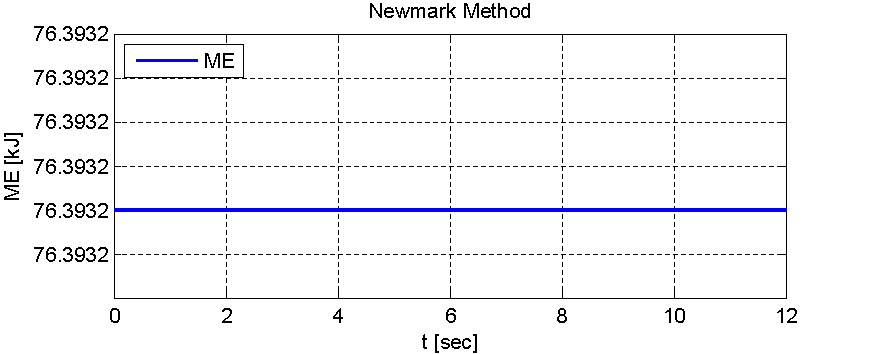
\includegraphics[width=\textwidth]{313_Newmark_mechen.pdf}}%
\\
\subfigure[][]{%
\label{fig:szabrezg_erek_newmark-b}%
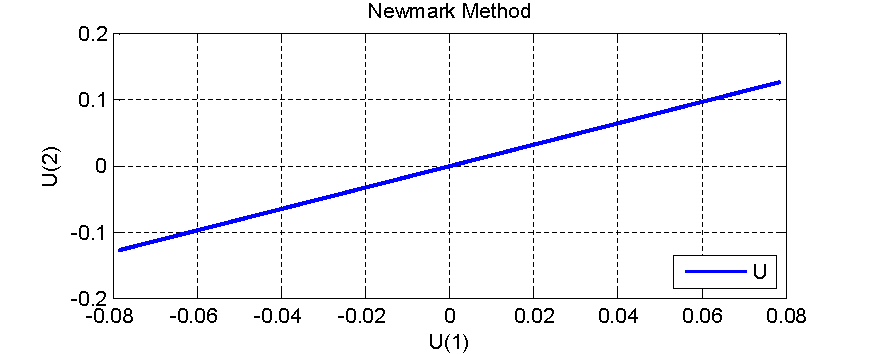
\includegraphics[width=\textwidth]{313_Newmark_elm.pdf}}%
\caption[A \ref{subsec:szabrezg} szabadrezgéses példa megoldásai Newmark módszerrel.]{A \ref{subsec:szabrezg} szabadrezgéses példa megoldásai  Newmark módszerrel:
\subref{fig:szabrezg_erek_newmark-a} a rendszer mechanikai energiája;
\subref{fig:szabrezg_erek_newmark-b} az elmozdulások fázistérben ábrázolva.}%
\label{fig:szabrezg_erek_newmark}
\end{figure}


 A grafikonokat elemezve láthatjuk, hogy az Euler-módszerrel az elmozdulások számítása elszáll, a rendszer mechanikai energiája minden határon túl nő, és az elmozdulások egymáshoz viszonyított előjele is hibás. A Runge-Kutta módszernél a csillapítás negatív előjelű a mechanikai energia növekszik, a Wilson-$\theta$ és HHT-$\alpha$ módszereknél pedig pozitív előjelű csillapítás érzékelhető. A periódusidő meghosszabbodása a Wilson-$\theta$ eljárásnál a legkisebb, és  Newmark,  HHT-$\alpha$, valamint CR algoritmusokkal számolva ehhez képest csak minimálisan növekszik. A legnagyobb meghosszabbodás a Runge-Kutta módszernél keletkezik.
 





\subsection{A nemlineáris időlépéses megoldó program eredményei statikus  probléma esetén}\label{subsec: nemlin eredmény stat}


A \ref{subsec:nemlinstat} statikus nemlineáris feladatban bemutatom, hogy a különböző $\xi$ értékek milyen mértékben befolyásolják az elmozdulások kialakulását. A \ref{fig:322_newmark_disp} ábrán az elmozdulás - idő függvények láthatók $\xi = 0.1, 0.5,$ és $1.1$ értékekre, a Newmark módszer elmozdulásos változatával számolva. A $\xi = 0.1$ értéknél (\ref{fig:322_newmark_disp-a} ábra) kialakul egy gyorsan lecsengő rezgés az állandósult érték körül. A $\xi = 0.5$ paraméter esetében (\ref{fig:322_newmark_disp-b} ábra) még kialakul rezgés (hiszen túlmegy a statikus helyzeten), de nagyon gyorsan lecseng. A $\xi = 1.1 > 1$ esetén (\ref{fig:322_newmark_disp-c} ábra) már nagy csillapításról beszélünk, ekkor nem alakul ki rezgés, és az elmozdulás értéke nem éri el az állandósult értéket.

A végső elmozdulás az első szinten $17 mm$, a második szinten pedig $23 mm$.  Az eredmények alapján a csillapítási tényezőre a  $\xi = 0,5$ értéket javaslom használni.

Az egyes módszerekkel számolt megoldások grafikonjait a Függelék \ref{sec:függ 322} pontja tartalmazza.


\begin{figure}%
\centering
\subfigure[][]{%
\label{fig:322_newmark_disp-a}%
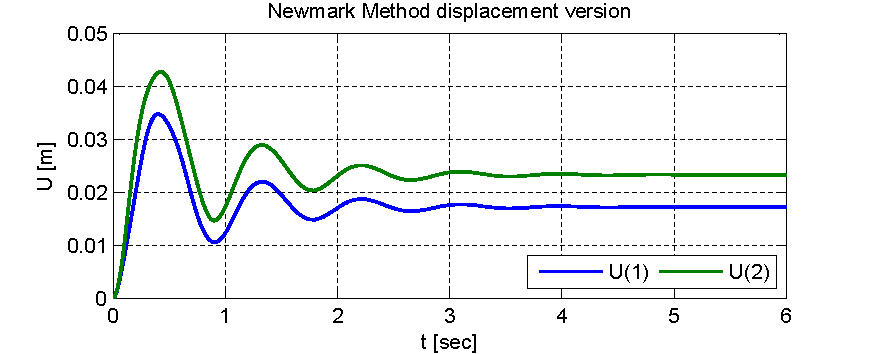
\includegraphics[width=0.75\textwidth]{322_newmark_disp_kszi_0_1.pdf}}%
\\
\subfigure[][]{%
\label{fig:322_newmark_disp-b}%
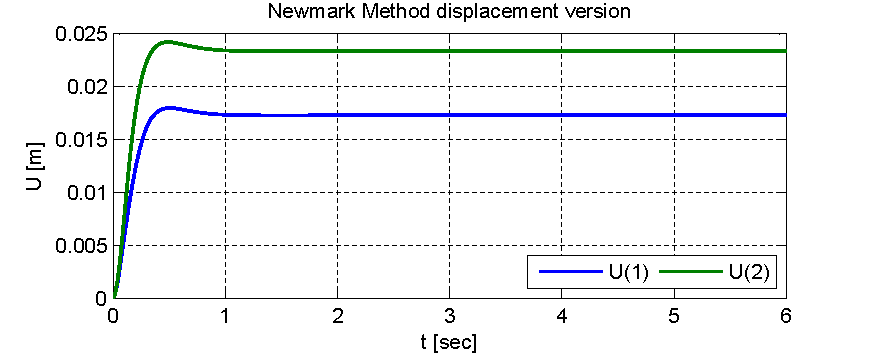
\includegraphics[width=0.75\textwidth]{322_newmark_disp_kszi_0_5.pdf}}%
\\
\subfigure[][]{%
\label{fig:322_newmark_disp-c}%
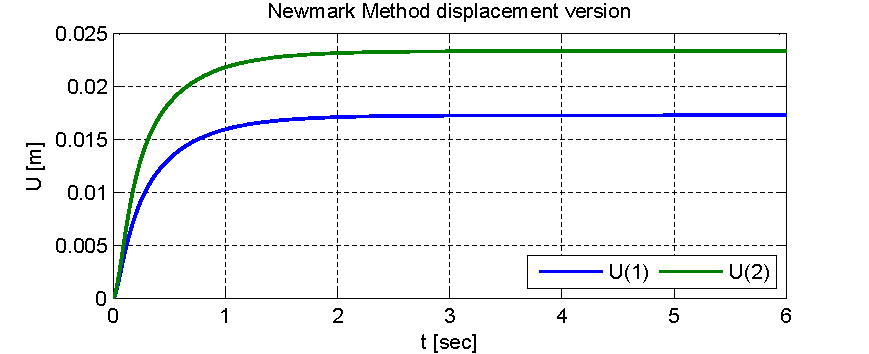
\includegraphics[width=0.75\textwidth]{322_newmark_disp_kszi_1_1.pdf}}%
\caption[A \ref{subsec:nemlinstat} statikus probléma elmozdulásai a Newmark módszer elmozdulásos változatával.]{A \ref{subsec:nemlinstat} statikus probléma elmozdulásai a Newmark módszer elmozdulásos változatával:
\subref{fig:322_newmark_disp-a} $\xi = 0.1$;
\subref{fig:322_newmark_disp-b} $\xi = 0.5$; 
\subref{fig:322_newmark_disp-c}  $\xi = 1.1$.}%
\label{fig:322_newmark_disp}%
\end{figure}
 


\subsection{A nemlineáris időlépéses megoldó program eredményei dinamikus probléma esetén}\label{subsec: nemlin eredmény din}

{\ }

A \ref{subsec:nemlindin} dinamikus nemlineáris feladat kapcsán  megfigyelhetjük a nemlineáris viselkedést. Most különböző terhelés hatására vizsgáljuk az elmozdulásokat. A tapasztalat szerint a teherfüggvényben az $\omega$  értéke meghatározza az időbeli lefutást.

A \ref{fig:323_newmark_disp_q_var_1} ábrán az elmozdulások láthatók az idő függvényében, különböző terhelések hatására a Newmark módszer elmozdulásos változatával számítva.  A grafikonról leolvasható, hogy a válasz a periodikus alakot megtalálja, viszont a maximum elmozdulás értékek nem a terhek arányát tükrözik. Az egyes módszerekkel számolt megoldások grafikonjait a Függelék \ref{sec:függ 323} pontja tartalmazza. 



\begin{figure}[h!p]
\centering
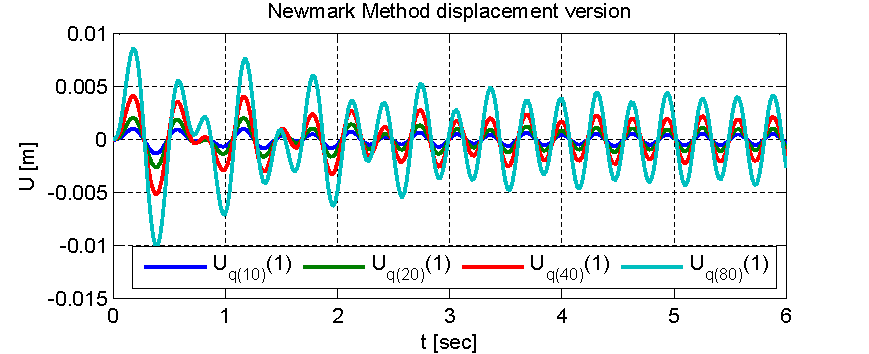
\includegraphics[width=0.75\textwidth]{323_Newmark_disp_q_var.pdf}
\caption{A \ref{subsec:nemlindin} dinamikus probléma megoldásai az első csomópontra a Newmark módszer elmozdulásos változatával különböző terhelésekre.}
\label{fig:323_newmark_disp_q_var_1}
\end{figure}
